\documentclass{article}
\usepackage{tikz}
\begin{document}

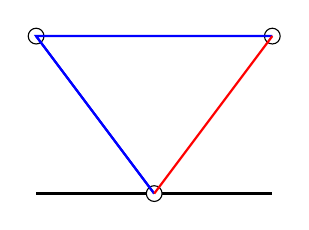
\begin{tikzpicture}
    % Draw the black horizontal line (ground)
    \draw[thick] (-1.5,0) -- (1.5,0);
    
    % Draw white circles at the top and bottom vertices
    \draw[fill=white] (0,0) circle (0.1);
    \draw[fill=white] (-1.5,2) circle (0.1);
    \draw[fill=white] (1.5,2) circle (0.1);
    
    % Draw the blue edges
    \draw[thick, blue] (-1.5,2) -- (0,0) -- (-1.5,2) -- (1.5,2); % Correction: Remove redundant path
    \draw[thick, blue] (-1.5,2) -- (1.5,2); % Top horizontal blue edge
    % Correction: Redraw the left blue edge clearly
    \draw[thick, blue] (-1.5,2) -- (0,0);
    
    % Draw the red edge
    \draw[thick, red] (0,0) -- (1.5,2);
    
    % Optional: Annotate the edges with labels if needed (not in the original image but can be considered)
    % \node[midway, above] at (-0.75,1) {Blue Edge};
    % \node[midway, above] at (0.75,1) {Red Edge};
\end{tikzpicture}

\end{document}